\begin{enumerate}
  \item 
  \begin{enumerate}
    \item La fonction $\Id_I$ et la fonction $E$ elle même sont des solutions évidentes de l'équation fonctionnelle $\mathcal{F}$.
    \item Soit $g$ définie dans $I$ et à valeurs dans $I$.\newline
Supposons $g$ solution de $\mathcal{F}$. Pour tout $n$ entier et tout réel $x$,
\[
  x \in \left[ n, n + 1 \right[ \Rightarrow n = E(x) = E(g(x)) \Rightarrow  g(x) \in \left[ n, n + 1 \right[
\]
Réciproquement, pour tout $x\geq 0$, notons $n = \lfloor x \rfloor$. L'implication signgifie que $\lfloor g(x) \rfloor = n$ c'est à dire $E \circ g (x) = E(x)$.
  \end{enumerate}

  \item
  \begin{enumerate}
    \item Comme $f$ est bijective, en composant à gauche par la bijection réciproque $f^{-1}$,
\[
\forall n \in \N,\;  f \circ E \circ f^{-1}(n) = n \Leftrightarrow E \circ f^{-1}(n) = f^{-1}(n) \Leftrightarrow f^{-1}(n) \in \N.
\]
    
    \item Ici $f$ est une bijection croissante de $I$ dans $I$. Elle est strictement croissante car elle est injective. Elle est continue car d'après un théorème de cours, comme $f$ est croissante, le fait que $f(I)$ soit un intervalle (ici $I$) entraine que $f$ est continue.\newline
    Supposons que $f \circ E \circ f^{-1}$ soit une solution de $\mathcal{F}$. Alors, d'après 1.b., 
    \[
\forall n \in \N,\;    f\circ E \circ f^{-1}(\left[ n, n + 1 \right[) \subset \left[ n, n + 1 \right[
\Rightarrow E \circ f^{-1}(\left[ n, n + 1 \right[) \subset f^{-1}(\left[ n, n + 1 \right[) .
    \]
en composant par la bijection réciproque $f^{-1}$. Comme $f^{-1}$ est continue et strictement croissante,
\[
  f^{-1}(\left[ n, n + 1 \right[) = \left[ f^{-1}(n), f^{-1}(n + 1) \right[.
\]
\begin{multline*}
  \text{Donc }E(\left[ f^{-1}(n), f^{-1}(n + 1) \right[) \subset \left[ f^{-1}(n), f^{-1}(n + 1) \right[ \\
  \Rightarrow f^{-1}(n) \leq E( f^{-1}(n))
  \Rightarrow f^{-1}(n) = E(f^{-1}(n))
  \Rightarrow f^{-1}(n) \in \N .
\end{multline*}

Réciproquement, supposons $f^{-1} (n) \in \N$ pour tout $n \in \N$. D'après 1.b., pour montrer que $f \circ E \circ f^{-1}$ est solution de $\mathcal{F}$, il suffit de montrer que 
\[
  \forall n \in \N, \;f\circ E \circ f^{-1}\left( \left[ n,n+1 \right[\right) \subset \left[ n, n+1 \right[.
\]
Pour tout réel $x$, l'encadrement $n \leq x < n + 1 $ entraine
\begin{multline*}
  f^{-1}(n) \leq f^{-1}(x) < f^{-1}(n+1) \; \text{ (car $f^{-1}$ strictement croissante)} \\
  \Rightarrow f^{-1}(n) \leq E(f^{-1}(x)) < f^{-1}(n+1) \; \text{ (car $f^{-1}(n)$ et $f^{-1}(n+1)$ entiers)} \\
  \Rightarrow n \leq f \circ E \circ f^{-1} (x) < n+1 \; \text{ (car $f$ strictement croissante)}.
\end{multline*}
  \end{enumerate}

  \item Application.
  \begin{enumerate}
    \item La fonction racine carrée est une bijection croissante de $I$ dans $I$. Prenons la comme fonction $f$ pour utiliser la question 2. Sa bijection réciproque est la fonction carrée restreinte à $I$. \'Evidemment, $f^{-1}(n) = n^2 \in \N$ pour tout $n\in \N$. On en déduit
\[
  E\circ f \circ E \circ f^{-1} = E 
  \Rightarrow E\circ f \circ E  = E \circ f
  \Rightarrow \left( \forall x \geq 0, \; \lfloor \sqrt{\lfloor x \rfloor}\rfloor = \lfloor \sqrt{x}\rfloor \right). 
\]
    \item La fonction $f$ définie par $f(x) = \frac{x + m}{n}$ vérifie les conditions de 2.b. avec $f^{-1}(y) = ny -m$ donc $f^{-1}(\N) \subset \N$. 
    \item De même pour $f(x) = \log_b(x)$ avec $f^{-1}(y) = b^y$. La relation est alors vérifiée si $f^{-1}(\N \setminus \left\lbrace 0,1 \right\rbrace) \subset \N$ donc en particulier pour $b$ naturel.
  \end{enumerate}

\begin{figure}[h!]
  \centering
  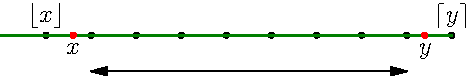
\includegraphics{Cracent_1.pdf}
  % Cracent_1.pdf: 156x3 px, 72dpi, 5.50x0.11 cm, bb=0 0 156 3
  \caption{Intervalle entier}
  \label{fig:Cracent_1}
\end{figure}
  
  \item
  \begin{enumerate}
    \item Soit $x < y$ réels. Notons $p = \min\left( \left] x, y \right[ \cap \Z \right)$ et $q = \max\left( \left] x, y \right[ \cap \Z \right)$. Alors 
\[
  \left] x, y \right[ \cap \Z = \llbracket p, q \rrbracket
\]
avec 
\[
\begin{aligned}
\left(x < p = (p-1) + 1 \text{ et } p-1 \leq x \right) &\Rightarrow p-1 = \lfloor x \rfloor \Rightarrow p = \lfloor x \rfloor +1 .\\
\left(q = (q+1) - 1 < y \text{ et } q + 1 \geq y \right) &\Rightarrow q+1 = \lceil y \rceil  \Rightarrow q = \lceil y \rceil -1 .
\end{aligned} 
\]
D'après l'égalité précédente, $\card\left(\left] x, y \right[ \cap \Z\right) = q - p +1$. Alors:
\[
  \begin{aligned}
    \left( q < y \text{ et } x < p \right) &\Rightarrow \card\left(\left] x, y \right[ \cap \Z\right) < y - x + 1 \\
    \left( q \geq y - 1 \text{ et } x \geq p -1 \right) &\Rightarrow \card\left(\left] x, y \right[ \cap \Z\right) \geq y - x -1
  \end{aligned}
\]

    \item Soit $0 \leq a < b \leq 1$ et $m \in \N$.\newline
    Quels sont les $k\in \N$ tels que $\lfloor \sqrt{k} \rfloor = m$ et $a < \sqrt{k} - \lfloor \sqrt{k} \rfloor < b$ ?\newline 
Comme $0 \leq a < b \leq 1$, ce sont les $k$ entiers tels que  
\[
  m + a < \sqrt{k} < m + b \Leftrightarrow (m+a)^2 < k < (m+b)^2
\]
c'est à dire $\left] (m+a)^2 , (m+b)^2 \right[ \cap \Z$.

    \item On veut montrer que la suite $(\sqrt{n} - \lfloor \sqrt{n} \rfloor)_{n \in \N}$ est bien répartie. Notons $\overline{n} = \lfloor \sqrt{n} \rfloor$.\newline
Soit $0 \leq a < b \leq 1$. Nommons $X_n$ l'ensemble des entiers $k$ entre $0$ et $n$ tels que 
\[
  a < \sqrt{k} - \lfloor \sqrt{k} \rfloor < b.
\]
Classons les $k \in X_n$ selon les valeurs de $\lfloor \sqrt{k} \rfloor$ qui est un entier $m$ quelconque dans $\llbracket 0, \overline{n}\rrbracket$. Nommons $X_{n,m}$ l'ensemble des $k$ tels que $\lfloor \sqrt{k} \rfloor = m$ et $a < \sqrt{k} - \lfloor \sqrt{k} \rfloor < b$.\newline
Alors $X_n$ est l'union disjointe de $X_{n,m}$ et 
\[
  \card(X_n) = \sum_{m=0}^{\overline{n}} \card(X_{n,m}).
\]
D'après les questions 4.b. et 4.c.,
\[
 (m+b)^2 - (m+a)^2 -1 \leq \card(X_{n,m}) < (m+b)^2 - (m+a)^2 + 1
\]
Comme $(m+b)^2 - (m+a)^2 = 2(b-a)m + b^2 - a^2$, on peut calculer la somme ce qui conduit à
\[
  2(b-a)\,\frac{\overline{n}(\overline{n}+1)}{2} + \overline{n}(b^2 - a^2 - 1) \leq \card(X_n) < 2(b-a)\,\frac{\overline{n}(\overline{n}+1)}{2} + \overline{n}(b^2 - a^2 + 1)
\]
Pour pouvoir conclure que la suite est bien répartie en utilisant le théorème d'encadrement pour les suites, il reste à montrer que 
\[
  (\frac{\overline{n}}{n})_{n\in \N^*}\rightarrow 0 \;\text{ et } \;(\frac{\overline{n}(\overline{n}+1)}{n})_{n\in \N^*}\rightarrow 1.
\]
On utilise encore le théorème d'encadrement
\[
  0 \leq \frac{\overline{n}}{n} \leq \frac{\sqrt{n}}{n} = \frac{1}{\sqrt{n}}\rightarrow0
\]
\[
  \underset{\rightarrow 1}{\underbrace{1 - \frac{1}{\sqrt{n}}}} = \frac{(\sqrt{n}-1)\sqrt{n}}{n}
  \leq \frac{\overline{n}(\overline{n}+1)}{n} 
  \leq \frac{\sqrt{n}(\sqrt{n}+1)}{n} = \underset{\rightarrow 1}{\underbrace{1 + \frac{1}{\sqrt{n}}}}.
\]

  \end{enumerate}

\end{enumerate}

